\documentclass[11pt]{article}

\usepackage{deauthor}
\usepackage{times,graphicx}

% user packages
\usepackage{todonotes}
\usepackage{pifont}
\newcommand{\cmark}{\ding{51}}
\newcommand{\xmark}{\ding{55}}
\usepackage{multirow}
\usepackage{booktabs}
\usepackage{graphicx}
\usepackage{subfig}
\usepackage{amsfonts}
\usepackage{amsmath}
\usepackage{amssymb}
\usepackage{booktabs}
\usepackage{pifont}
\newcommand{\ulnewnew}[1]{\underline{#1}}
\usepackage{makecell}
\usepackage{multirow}
\usepackage{multicol}
\usepackage{cancel}
\newcommand{\mr}[3]{\multirow{#1}{#2}{#3}}
\newcommand{\mc}[3]{\multicolumn{#1}{#2}{#3}}
\renewcommand{\mathbf}[1]{\boldsymbol{#1}}
\usepackage{wrapfig}
\def\modelname{HyCLID}
\def\figwidth{0.28}
\def\detailfigwidth{0.31}
\def\visualfigwidth{0.31}
\newcommand{\tabincell}[2]{\begin{tabular}{@{}#1@{}}#2\end{tabular}}

\usepackage{url}

\title{Graph Contrastive Learning: An Odyssey towards Generalizable, Scalable and Principled Representation Learning on Graphs}
\author{
    Yan Han$^{\dagger}$ \hspace{1em} Yuning You$^{\ddagger}$ \hspace{1em} Wenqing Zheng$^{\dagger}$ \hspace{1em} Scott Hoang$^{\dagger}$ \hspace{1em} Tianxin Wei$^{\S}$ \\
    Majdi Hassan$^{\P}$ \hspace{1em} Tianlong Chen$^{\dagger}$ \hspace{1em} Ying Ding$^{\dagger}$ \hspace{1em} Yang Shen$^{\ddagger}$ \hspace{1em} Zhangyang Wang$^{\dagger}$ \\
    \\
    $^{\dagger}$University of Texas at Austin \\
    \texttt{\small\{yh9442, w.zheng, hoangd, tianlong.chen, atlaswang\}@utexas.edu} \\
    \texttt{\small ying.ding@austin.utexas.edu} \\
    \\
    $^{\ddagger}$Texas A\&M University \\
    \texttt{\small\{yuning.you, yshen\}@tamu.edu} \\
    \\
    $^{\S}$University of Illinois Urbana-Champaign \\
    \texttt{\small twei10@illinois.edu} \\
    \\
    $^{\P}$AbbVie \\
    \texttt{\small majdi.mhas@gmail.com}
}


% unnecessary commands
\usepackage{paralist}
\newcommand{\entity}{\mathcal{E}}
\newcommand{\relation}{\mathcal{R}}
\newcommand{\lang}{\mathcal{L}}
\newcommand{\model}{\mathcal{M}}
\newcommand{\term}{\mathcal{T}}
\newcommand{\kgnew}{\mathcal{KG}}

\begin{document}
\maketitle
\renewcommand\thesection{\arabic{section}}
\setcounter{section}{0}
\setcounter{figure}{0}
\setcounter{table}{0}

\begin{abstract}
Graph Contrastive Learning (GCL), an uprising regime of learning representations of graph-structured data, has gained significant attention in recent years. At its core, GCL leverages the idea of comparing different views of a graph to learn representations that capture desirable characteristics of the graph structures. GCL has been applied to a wide range of graph-structured data, including attributed graphs, multi-relational graphs, temporal graphs, hierarchical graphs, heterogeneous graphs, and hypergraphs. The learned graph representations yield predictive performance that generalizes well in various downstream tasks at the node, link, and graph levels, and can scale up to graphs with millions of nodes. In this paper, we present a review of representative GCL approaches with a major emphasis on our own recent efforts. Beginning with the original GCL approach with ad-hoc view generation and simple homogeneous graphs, we demonstrate how the framework can be further extended to more complex heterogeneous graphs and hypergraphs, as well as improved via principled view generation towards generalizability, fairness, interpretability, and other aspects. Theoretical explorations are covered at the end. In conclusion, we discuss the future prospects and ongoing challenges in the field of GCL.
\end{abstract}

\section{Introduction}  
\label{sec:1}
Graph-structured data are ubiquitous in various real-world applications, including social networks, biological networks, transportation systems, and recommender systems \cite{kipf_semi_supervised_2017, hamilton2017inductive, wu_graph_2020}. The analysis and learning from graph data have gained increasing importance as they can unveil hidden patterns and relationships, thereby enhancing decision-making in practical scenarios. In recent years, graph contrastive learning (GCL) has emerged as a promising approach for graph representation learning. GCL has demonstrated remarkable success in capturing the underlying structural properties of graphs and achieving generalized predictive performance.

The key concept behind GCL, inspired by image representation learning \cite{chen2020simple}, is simple yet effective: comparing different views of a graph to learn representations that encapsulate its desirable structural properties, which can scale up to large graphs. However, determining what and how to contrast presents a non-trivial challenge when it comes to graph data. Unlike images, graph data exhibit high heterogeneity across applications in terms of both semantics and graph types (e.g., social networks versus molecular scaffolds). Consequently, achieving a universally beneficial design is exceedingly difficult.

In this paper, we present a comprehensive review of various GCL approaches, with a particular focus on our recent contributions. We start from introducing the vanilla GCL approach, known as vanilla GCL, which involves the utilization of ad-hoc view generation and primarily targets simple homogeneous graphs. Subsequently, we systematically explore the extensions of the GCL framework to accommodate more intricate heterogeneous graphs and hypergraphs. This involves the integration of principled view generation techniques to enhance generalizability, fairness, interpretability, and other important aspects. We in addition cover the preliminary but critical investigations of the theoretical aspects, providing valuable insights into the underlying mechanisms and potential limitations of GCL. We conclude the paper by discussing future prospects and open challenges in the GCL field, including potential directions for further research and development in this area.


\section{GCL Approaches and Graph Types}
\label{sec:gcl_approaches_and_graph_types}
\subsection{Homogeneous Graphs}
\label{sec:homogeneous_graphs}
A homogeneous graph, denoted as $\mathcal{G} = \{\mathcal{V}, \mathcal{E}\} \in \mathbb{G}$, is characterized by a set of vertices $\mathcal{V} = \{v_1, ..., v_{|\mathcal{V}|}\}$ and a set of edges $\mathcal{E} = \{(v_i, v_j) | v_i, v_j \in \mathcal{V}\}$. In different contexts, each vertex and edge can be associated with specific attributes for feature representation. For example, in social networks \cite{mitchell1974social}, vertices may correspond to user side-information and edges to connections, while in molecular graphs \cite{clark2012molecular}, vertices may represent atoms and edges may represent bond types. These attributes can be mapped to vectorial representations of dimension $D$ using graph neural networks (GNNs) \cite{kipf2016semi, velivckovic2017graph, xu2018powerful}. Thus, GNNs can be represented as $f_\theta: \mathbb{G} \rightarrow \mathbb{R}^D$, where $\theta$ denotes the parameters of the GNN, enabling downstream utility.

In the supervised learning setting, the annotated dataset $\mathcal{D}_\mathrm{lab} = \{(\mathcal{G}_1, \mathcal{Y}_1), ...\}$ is provided, where machine learning models, such as GNNs, can be trained to make predictions on new, unseen data. However, the effectiveness of supervised learning is hindered by the challenge of limited graph labels \cite{mitchell2007machine}. One dominant solution to address the challenge is to employ self-supervised learning, where models are pre-trained on large-scale unlabeled data \cite{chen2020simple, devlin2018bert}. The rationale behind this approach is well-appropriate principled objectives could enhance their generalizability. Fortunately, accessing unlabeled datasets $\mathcal{D}_\mathrm{unlab} = \{\mathcal{G}_1, ...\}$ for graphs is often viable. A key question then arises: \textit{how can self-supervised objectives be designed specifically for graph-structured data?}

Among the various self-supervised tasks for graphs (for a more comprehensive review, please refer to \cite{xie2022self, liu2022graph}), graph contrastive learning (GCL) \cite{you2020graph, velickovic2019deep, zhu2020deep, hassani2020contrastive, sun2019infograph, qiu2020gcc} stands out due to its consistently generalizable performance across diverse applications. The fundamental concept of GCL is to compare different views of a graph to learn representations that capture the desired structural properties of the graph (refer to Figure \ref{fig:graphcl} for the overall pipeline). In GCL, prior knowledge is explicitly incorporated into graph neural networks (GNNs) through the construction of graph views. Consequently, the primary focus of GCL research is to investigate effective methods for constructing graph views that incorporate appropriate inductive biases.
The training of GCL with a batch of graph samples $\{\mathcal{G}_1, ..., \mathcal{G}_N\}$ is then formulated using the NT-Xent loss \cite{chen2020simple} as follows:
\begin{equation}
    \min_{\theta, \phi} \ \mathcal{L}_\mathrm{GCL}(\theta, \phi) = \min_{\theta, \phi} \ - \frac{1}{N} \sum_{n=1}^N \log \frac{\exp\left(\mathrm{sim}\left(g_\phi \circ f_\theta (\tilde{\mathcal{G}}_{n,1}), g_\phi \circ f_\theta (\tilde{\mathcal{G}}_{n,2})\right)  / \tau\right)}{\sum_{n'=1, n' \neq n}^N \exp\left(\mathrm{sim}\left(g_\phi \circ f_\theta (\tilde{\mathcal{G}}_{n,1}), g_\phi \circ f_\theta (\tilde{\mathcal{G}}_{n',2})\right)  / \tau\right)}
\end{equation}
where $g_\phi(\cdot)$ represents the projection head implemented as a multi-layer perceptron \cite{chen2020simple}, $\tilde{\mathcal{G}}_{n,i} = h_i(\mathcal{G}_n)$ denotes the contrastive view of $\mathcal{G}_n$, $\mathcal{G}'_n$ is treated as the negative sample, $\mathrm{sim}(\cdot, \cdot)$ is the similarity function (typically implemented using cosine similarity $\mathrm{sim}(z_1, z_2) = z_1^\mathsf{T} z_2 / \lVert z_1 \rVert \lVert z_2 \rVert$), and $\tau \in \mathbb{R}_{>0}$ is the temperature parameter.
\begin{figure}[t] 
    \centering 
    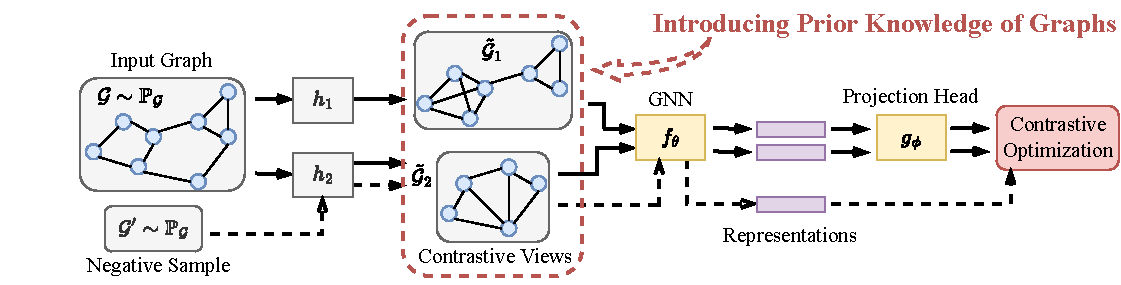
\includegraphics[width=1\linewidth]{submissions/Yan2023/figures/graphcl.drawio.pdf}
    \caption{The generic pipeline of homogeneous GCL.} 
    \label{fig:graphcl}
\end{figure}

\begin{wraptable}{r}{0.6\textwidth}
 \vspace{-0.5em}
 \caption{Four generic augmentation strategies (in the spatial domain) with the corresponding underlying inductive bias.} \label{tab:data_augmentation}
 \vspace{-0.5em}
 \centering
 \resizebox{0.6\textwidth}{!}{
 \begin{tabular}{c | c c c } 
  \toprule
  Data Augmentation & Type & Underlying Prior \\
  \midrule
  Node dropping & Nodes, edges & Vertex missing does not alter semantics. \\
  Edge perturbation & Edges & Semantic robustness against connectivity variations. \\
  Attribute masking & Nodes & Semantic robustness against partial attribute loss. \\
  Subgraph & Nodes, edges & Local structure can provide hints to full semantics. \\
  \bottomrule
 \end{tabular}}
 \vspace{-0.5em}
\end{wraptable}
\noindent
\textbf{Graph data augmentations for view construction.}
A well-established approach to construct contrastive views is through graph data augmentations \cite{you2020graph, zhu2021graph, ding2022data, zhao2021data, zhou2020data, marrium2022data}, which effectively introduce inductive biases specific to the target applications. For example, in one of the earliest works \cite{you2020graph}, four generic graph augmentations are designed, as shown in Table \ref{tab:data_augmentation}, each with an underlying prior incorporated. These augmentations operate in the spatial domain and include node dropping, edge perturbation, attribute masking, and subgraph transformations, the resulting views of which capture different aspects of the graph's semantics.

In addition to augmentations in the spatial domain, spectral augmentations have been proposed for graph data, leveraging the graph spectrum where the semantic information is more accessible \cite{ghose2023spectral, zhang2022spectral, lin2022spectral}. Furthermore, some works explore augmentations in the latent space implicitly learned by the model \cite{xie2022self2, kong2020flag, verma2021graphmix}, which is believed to better capture the underlying semantics. Other approaches focus on augmenting specific graph model-based parameters, such as graphons \cite{han2022g, ruiz2020graphon} or contextual stochastic block models (CSBMs) \cite{wei2022understanding}, based on the explicit downstream data generation assumptions.

Overall, the choice of graph data augmentations plays a crucial role in constructing effective contrastive views and capturing the desired inductive biases for the specific graph-structured data. In certain designated applications, augmentations can be specifically designed to cater to the unique characteristics of the data. For example, small molecules have been shown to benefit from motif-based \cite{wang2022improving, fang2022molecular} or energy-guided \cite{liu2022molecular} perturbations. Similarly, protein structures can be augmented through cropping while preserving consecutive amino-acid sequences \cite{zhang2022protein, you2022cross}. The construction of effective graph views for contrastive learning, which are robust across diverse domains or exhibit strong generalizability in specific applications, remains an active area of research.

\subsection{Heterogeneous Graphs}
A heterogeneous graph is defined as $\mathcal{G} = \{\mathcal{V}, \mathcal{E}, \mathcal{T_V}, \mathcal{T_E}\} \in \mathbb{G}$, where $\mathcal{V} = \{v_1, ..., v_{|\mathcal{V}|}\}$ represents the set of vertices, $\mathcal{E} = \{(v_i, v_j) | v_i, v_j \in \mathcal{V}\}$ denotes the set of edges, $\mathcal{T_V}$ denotes the set of different vertex types, and $\mathcal{T_E}$ represents the set of different edge types. In various contexts, each vertex and edge in a heterogeneous graph may be associated with specific attributes (e.g., user profiles and relationships in social networks \cite{sun2012mining}, or gene expressions and regulatory interactions in biological networks \cite{peng2021end}), which serve as features for graph learning.

Differing from homogeneous graphs, the complicated relations in heterogeneous graphs are more effectively captured by meta-paths.
A meta-path \cite{sun2011pathsim, dong2017metapath2vec} $P$ is a path that connects multiple nodes in the form of $A_1\stackrel{R_1}{\longrightarrow} A_2 \stackrel{R_2}{\longrightarrow}\dots\stackrel{R_l}{\longrightarrow}A_{l+1}$ (abbreviated as $A_1A_2\dots A_{l+1}$). It describes a composition of different relations $R_1, R_2, \dots, R_l$ that link objects $A_1$ and $A_{l+1}$. For example, in the heterogeneous graph shown in Figure \ref{heterocl}(a), there are two different meta-paths: Movie-Director-Movie (MDM), which represents the co-director relation between two movies, and Movie-Actor-Movie (MAM), which represents the co-actor relation between two movies. Different meta-paths reveal diverse semantics and guide the connection of even distant objects based on their semantic similarities. Utilizing meta-paths as prior knowledge in positive sampling ensures that the selected candidates are semantically related to some extent.

\begin{figure}
  \centering
  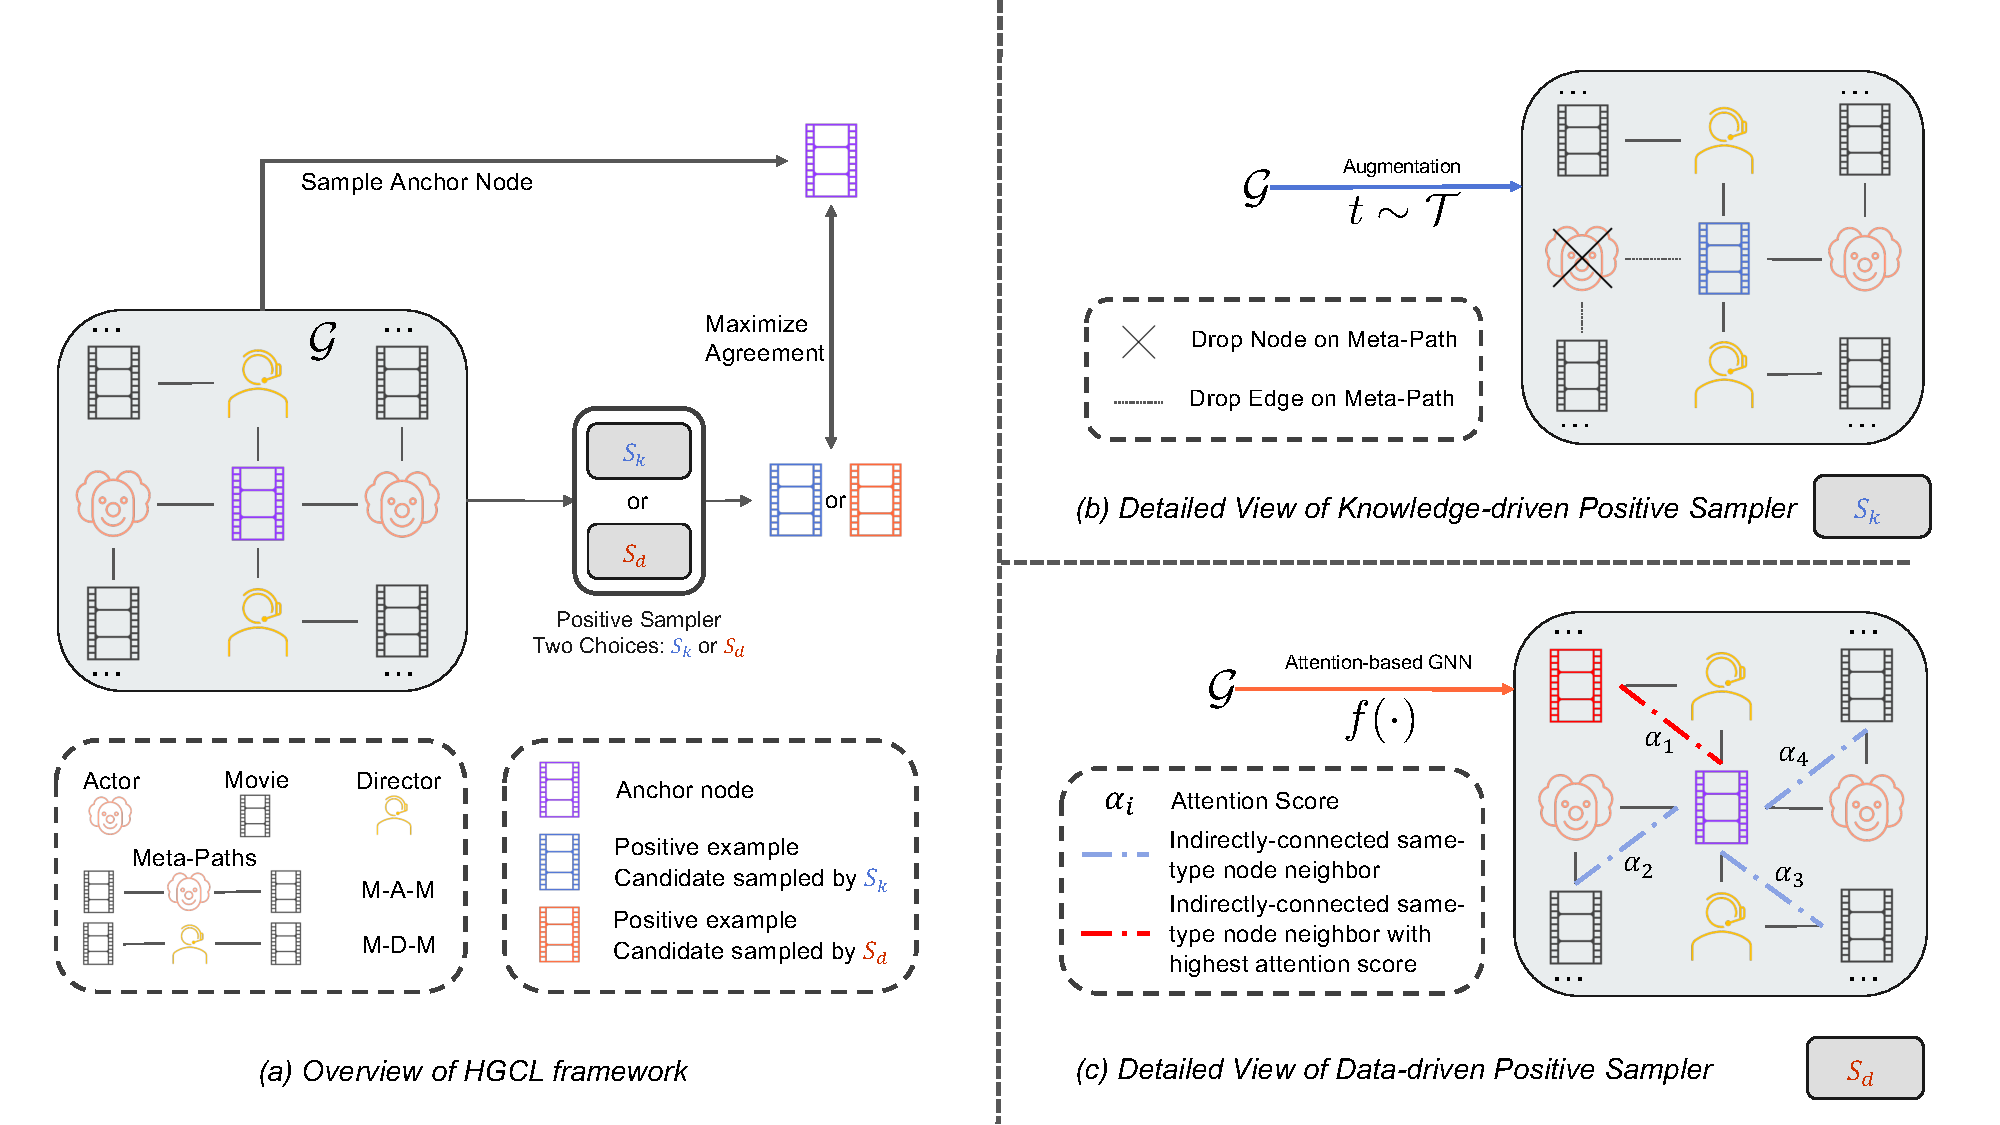
\includegraphics[width=0.95\linewidth]{submissions/Yan2023/figures/heterographcl.pdf}
  \caption{HGCL framework: (a) \textbf{Overview}: Anchor node $u$ and positive example node $v$ in a heterogeneous graph $\mathcal{G}$ are processed with a GNN backbone and projection head using a contrastive loss. (b) \textbf{$S_k$ (knowledge-driven)}: Pre-defined meta-paths guide positive example node $v_k$ generation. (c) \textbf{$S_d$ (data-driven)}: GNN-based encoder with attention module generates positive example node $v_d$.}
  \label{heterocl}
\end{figure}

Heterogeneous graph contrastive learning (HGCL) has witnessed significant progress through various methods. HeCo \cite{wang2021self} utilizes meta-path-based random walks for self-supervised learning, while STENCIL \cite{zhu2022structure} employs structural templates to encode neighborhood information. HGCLR \cite{chen2023heterogeneous} learns embeddings by contrasting multiple meta-path-derived views, and CPT-HG \cite{jiang2021contrastive} captures node relations through pairwise contrastive learning. MVSE \cite{zhao2021multi} combines intra-view and inter-view contrastive learning tasks using different meta-path-based views. Generally, contrastive learning methods can be classified into two categories: \textbf{knowledge-driven} and \textbf{data-driven}, with a primary focus on generating positive views.

\textbf{Knowledge-driven views.}
As illustrated in Figure \ref{heterocl}(b), the framework leverages meta-paths to drop nodes or perturb edges, resulting in related views. This strategy shares similarities with homogeneous graphs, with the key difference being that the augmentation in heterogeneous graphs depends on meta-paths.

\textbf{Data-driven views.}
As demonstrated in Figure \ref{heterocl}(c), data-driven methods rely on attention mechanisms employed in graph neural networks \cite{wang2019heterogeneous, velickovic2018graph, Fu_2020}. The attention score, $e_{ij}$, of node $j$'s embedding to node $i$ serves for the learnable sampling distribution as:
\begin{align}
    e_{ij} = \textrm{LeakyReLU}(a (Wh_i||Wh_j)), \quad \alpha_{ij} = \textrm{softmax}_j (e_{ij}) = \frac{\exp (e_{ij})}{\sum_{k\in \mathcal{N}i}\exp (e_{ik})}
\end{align}

To ensure differentiability in selecting the positive example $\textbf{v}^+$, the Gumbel-Softmax trick \cite{jang2016categorical} is introduced, using the softmax function as a continuous, differentiable approximation (Gumbel-Softmax trick), facilitating joint updates of the learned sampling distribution $p_d$ during training, resulting in a dynamic and adaptive contrastive learning framework:

\begin{equation}\label{gs}
v^+_j = \frac{\exp ((\log(\alpha_{ij}) + g_j)/\tau)}{\sum_{m=1, m\neq i}^k \exp (\log(\alpha_{im}) + g_m)/\tau)}, \ \textrm{for} \ j = 1,\cdots, \cancel{i},\cdots, k
\end{equation}

\begin{figure}[t] 
\centering
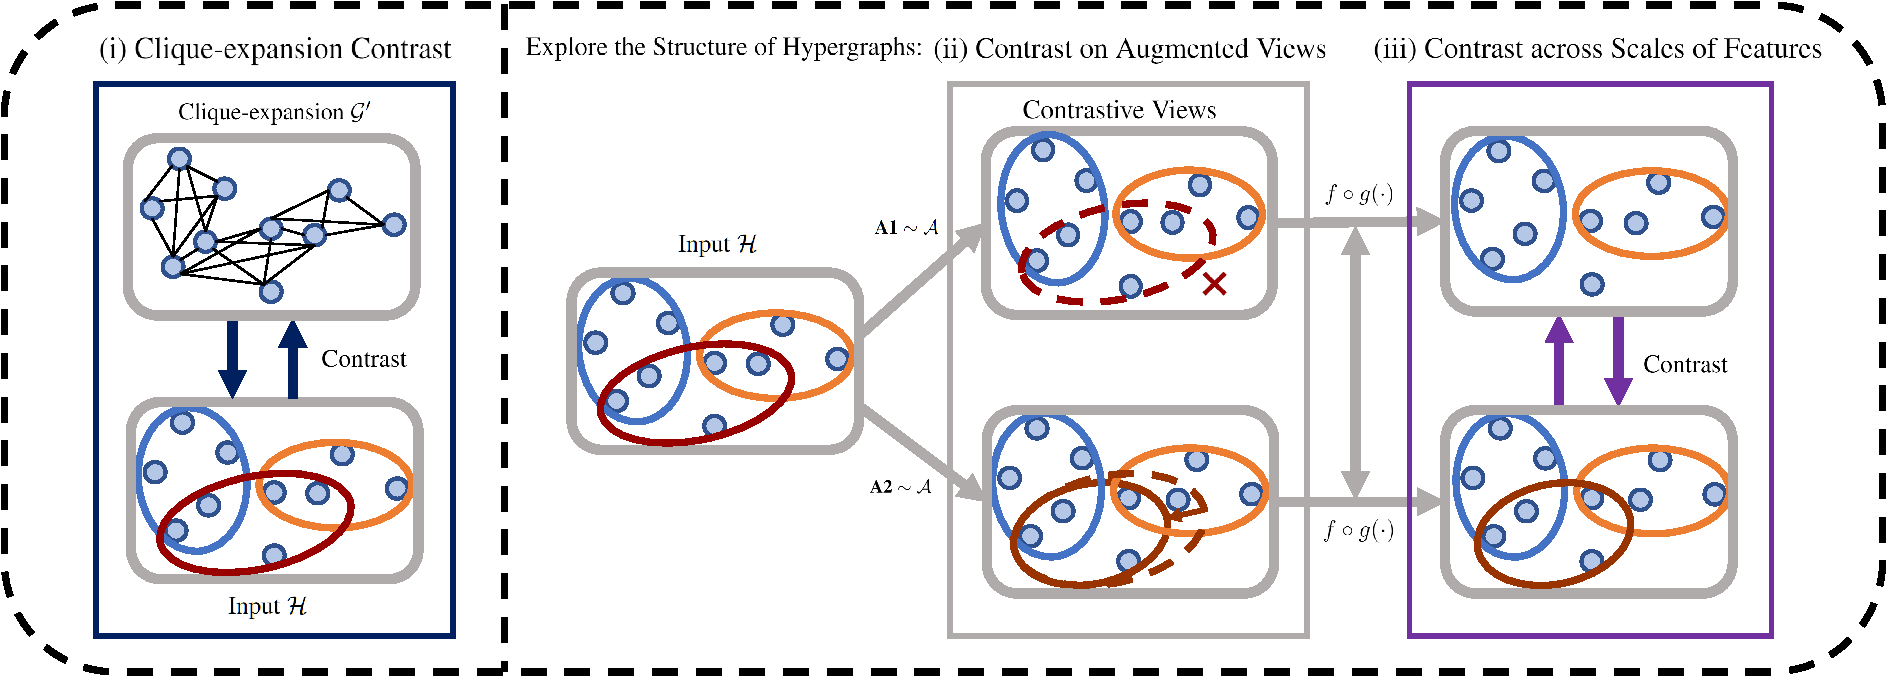
\includegraphics[width=1\linewidth]{submissions/Yan2023/figures/hypergraphcl.pdf}
\caption{Three major lines of HyperGCL pipelines: (i) clique-expansion contrast, (ii) contrasting on augmented hypergraph views, and (iii) contrasting across scales of augmented hypergraph features.
}
\label{fig:hyper_frame}
\end{figure}

\begin{wraptable}{r}{0.3\textwidth}
\vspace{-1em}
 \caption{Five generic augmentation operations for HyperGCL.} \label{tab:hypergraph_operations}
 \vspace{-0.5em}
 \centering
 \resizebox{0.3\textwidth}{!}{
 \begin{tabular}{c c c c } 
  \toprule
    Hypergraph Augmentations \\ \midrule
    Na\"ive Hyperedge Perturbation \\
    Generalized Hyperedge Perturbation      \\
    Vertex Dropping        \\
    Attribute Masking      \\
    Subgraph               \\
    Generative Augmentation \\ \bottomrule
 \end{tabular}}
\end{wraptable}

\subsection{Hypergraphs}
Hypergraphs extend the concept of homogeneous and heterogeneous graphs by allowing many-body interactions across nodes, represented by hyperedges. They have attracted significant attention in the research community \cite{feng2019hypergraph, yadati2019hypergcn, chien2021you}. A hypergraph is denoted as $\mathcal{H} = \{ \mathcal{V},\mathcal{E} \} \in \mathbb{H}$, where $\mathcal{V}=\{v_1,...,v_{|\mathcal{V}|}\}$ is the set of vertices and $\mathcal{E}=\{e_1,...,e_{|\mathcal{E}|}\}$ is the set of hyperedges. Each hyperedge $e_n = \{ v_1,...,v_{|e_n|} \}$ represents a higher-order interaction among a set of vertices. Hypergraph neural networks (HyperGNNs) \cite{feng2019hypergraph, yadati2019hypergcn, chien2021you} have been proposed as state-of-the-art approaches to encode such complex structures, mapping the hypergraph to a $D$-dimensional latent space via $f: \mathbb{H} \rightarrow \mathbb{R}^D$ using higher-order message passing. For contrastive learning, a projection head $h(\cdot)$ is applied to $f(\cdot)$. Currently, most hypergraph contrastive learning (HyperGCL) methods focus on node-level applications.

When dealing with complex relationships in hypergraphs, the challenge is how to construct contrastive views for hypergraphs. However, building effective hypergraph views is non-trivial due to the overly complicated topology of hypergraphs. Unlike graphs, where there are $\binom{N}{2}$ possibilities for one edge with $N$ vertices, hyperedges in hypergraphs can have $2^N$ possibilities. To address this challenge, three lines of methods have emerged in HyperGCL research, which focus on (i) clique-expansion contrast, (ii) hypergraph view generation, and (iii) hypergraph objective augmentation, as summarized in Figure \ref{fig:hyper_frame}.

\textbf{Clique-expansion contrast.}
The first line of HyperGCL methods contrasts the representations of hypergraphs with clique-expansion views \cite{xia2022hypergraph, cai2022hypergraph}. This method is intuitive but computationally expensive in terms of time and memory, as it requires optimizing multiple neural networks of different modalities. Additionally, contrasting between clique expansion poses the risk of losing higher-order awareness by bringing the representations of hypergraphs and graphs closer together \cite{wei2022augmentations}.

\textbf{Contrasting on augmented hypergraph views.}
The second line of methods explores the structure of hypergraphs itself to construct contrastive views \cite{wei2022augmentations}. They assess whether generic augmentations are suitable for HyperGCL. Since hypergraphs are composed of hyperedges and vertices, they propose two strategies to augment hyperedges: direct perturbation on hyperedges and perturbation on the ``edges'' between hyperedges and vertices in the converted bipartite graph. To augment vertices, they adopt three schemes: vertex dropping, attribute masking, and subgraph, which are borrowed from graph-structured data augmentations \cite{you2020graph}. Their findings show that while vertex augmentations benefit graphs more, hypergraphs mostly benefit from hyperedge augmentations, revealing that higher-order information encoded in hyperedges is usually more downstream-relevant than information in vertices.

\textbf{Contrasting across scales of augmented hypergraph features.}
The last line of methods \cite{lee2022m, song2023chgnn} focuses on contrasting augmented features beyond the node-level. The main idea is to perform multi-level contrast, aiming to maximize the agreement between the same node, the node members of the same hyperedge, and each hyperedge and its node members in two augmented views. This approach expects that complementary information can be captured from different views to enhance HyperGCL.

\subsection{Principled Graph Views for Contrastive Learning}
The construction of appropriate contrastive views is crucial in GCL, but it often relies on empirical rules of thumb, which can vary significantly depending on the nature of the graph dataset. Therefore, the question arises: \textit{could we develop principled ways to construct graph views for contrastive learning?} The answer lies in two folds: defining the space of GCL views and formulating principles to search within that space (Figure \ref{fig:principle}).

\begin{wrapfigure}{r}{0.6\textwidth}
  \vspace{-2em}
  \begin{center}
    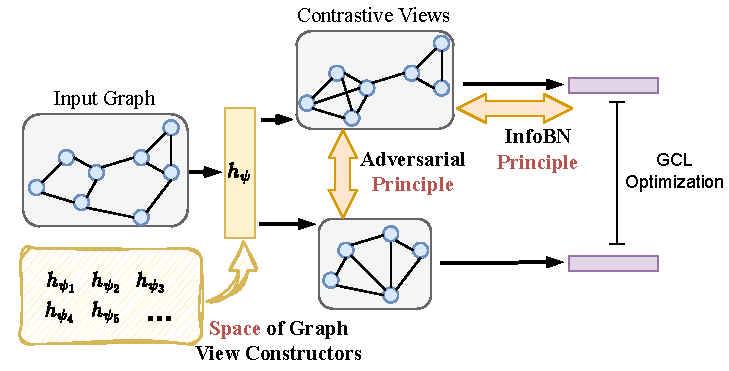
\includegraphics[width=0.6\textwidth]{submissions/Yan2023/figures/principles.drawio.pdf}
  \end{center}
  \vspace{-1.5em}
  \caption{Two indispensable steps for principled graph view construction: defining view space and formulating search principles.} \label{fig:principle}
  \vspace{-1em}
\end{wrapfigure}

\textbf{Space of graph contrastive views.}
Defining a good search space is essential for well-behaved search algorithms. The view constructor can be represented by a mapping function $h_\psi: \mathbb{G} \rightarrow \tilde{\mathbb{G}}$, where $\tilde{\mathcal{G}} = h_\psi(\mathcal{G})$ and $\psi$ represents the parameters of the mapping function. The search space is defined on this family of functions, specifically on the parameters $\psi$. Various approaches have been proposed to construct the function space, such as using learnable sampling distributions combined with prefabricated graph augmentation functions \cite{you2021graph}, masking operators on topology or node features \cite{zhu2021graph, suresh2021adversarial}, and training graph generative models to define the augmentation space in a data-driven manner \cite{you2022bringing, yin2022autogcl}. While the construction of search spaces is domain-agnostic, there is a need for further research to explore how to construct search spaces tailored to specific applications, e.g., in molecular graph analysis, chemical knowledge can be incorporated to define the graph augmentation functions. Future research can focus on customizing the search space construction to the characteristics of the target application.

\textbf{Principles for view searching.}
The choice of graph contrastive views can be sensitive to different datasets in GCL. However, evidence shows that views derived from certain principles, conditioned on the dataset, provide more robust benefits. View searching can be formulated as a bi-level optimization problem, where the upper-level optimization aims to minimize the GCL loss with respect to the parameters $\theta$ and $\phi$, while the lower-level optimization finds the optimal parameters $\psi^*$ that minimize a principled objective $\mathcal{L}_\mathrm{Principle}$. Various principles have been proposed for view construction. For example, adversarial training can enforce GCL to optimize on ``difficult'' views \cite{you2021graph}, leveraging graph properties can guide the view construction \cite{zhu2021graph}, and the information bottleneck principle can eliminate superficial features from raw graph data \cite{you2022bringing, suresh2021adversarial, xu2021infogcl}. Future research can focus on unifying different principles and understanding the relationships among them. Additionally, theoretical analysis to bridge principled view construction and downstream performance is needed for further development.

\subsection{Principled View towards Interpretability and Fairness}
While graph contrastive learning has shown success in various tasks, fairness and interpretability are important aspects that have received less attention in this area. In this section, we discuss the principled view for fairness and interpretability in graph contrastive learning, highlighting recent studies.

\textbf{Fairness.} Fairness in graph representation learning is crucial to prevent biased results, especially towards underrepresented groups. Graph contrastive learning methods can benefit from incorporating fairness-aware data augmentations to promote fair and unbiased representations. Studies such as Graphair \cite{ling2023learning}, as well as other approaches \cite{kose2022fair, kose2022fair2}, propose fairness-aware data augmentations that are learned from data. These augmentations, which can be integrated into graph contrastive learning frameworks, aim to mitigate sensitive information while preserving other useful information. By doing so, they improve the fairness-accuracy trade-off performance in various node classification datasets, leading to more equitable graph contrastive learning outcomes.

\textbf{Interpretability.} Interpretability is another important aspect of graph contrastive learning, as it helps users understand and trust the decisions made by graph neural networks (GNNs). Task-Agnostic GNN Explainer (TAGE) \cite{xie2022task} is a self-supervised, task-independent explanation approach that can be applied to GNNs used in graph contrastive learning. TAGE enables the explanation of GNN embedding models with unseen downstream tasks and allows efficient explanation of multitask models. Integrating TAGE into graph contrastive learning frameworks can significantly enhance their explanation efficiency while achieving similar or better explanation quality than existing state-of-the-art GNN explanation methods.

Another approach to improve the interpretability of GNNs in graph contrastive learning is to focus on their reasoning capabilities. Existing neural reasoners often struggle with out-of-distribution (OOD) test data featuring larger input sizes. A recent study \cite{bevilacqua2023neural} proposes data augmentation procedures that leverage causal frameworks to develop self-supervised objectives, which can also be applied to graph contrastive learning. By incorporating these data augmentation procedures into graph contrastive learning, the OOD generalization capabilities of the reasoner can be improved, resulting in better performance on OOD test data.

In summary, enhancing fairness and interpretability in graph contrastive learning is crucial for developing trustworthy and unbiased node representations. By incorporating fairness-aware data augmentations, self-supervised objectives, and interpretable explanation methods, we can create more robust and equitable graph contrastive learning frameworks that remain interpretable and generalizable across various application domains.

\subsection{Theoretical Exploration}
Although numerous algorithms and principles have been developed for GCL pretraining, the explicit theoretical connection between pretraining and downstream fine-tuning performance still lags behind. The gap between pretraining and fine-tuning performance can be attributed to several factors, including the misalignment between the optimization objectives of pretraining and fine-tuning, the discrepancy between the data distributions used in pretraining and fine-tuning, and the inductive biases encoded in neural networks. While the latter two factors have been more heavily studied in graph out-of-distribution generation \cite{bevilacqua2021size, you2023graph}, little work has been done to analyze the sources of error arising from the misalignment between pretraining and fine-tuning optimization objectives, especially in the context of GCL.

One major challenge in analyzing the misalignment between pretraining and fine-tuning in GCL is the diverse range of downstream applications for graph-structured data. Unlike Euclidean data, which has more standardized downstream tasks such as image classification \cite{du2020few, haochen2021provable}, graph-structured data is used in a wide range of applications, from molecule generation to social network analysis. This diversity makes it difficult to establish appropriate assumptions about downstream data distributions for analysis.

In a recent study, Trivedi et al. \cite{trivedi2022analyzing} attempted to bridge the gap between pretraining and fine-tuning in GCL by assuming a highly generic ``label-preserving'' behavior of graph views. They justified this assumption through the use of graph edit distances between contrastive views and label-preserved samples, which measure the similarity between two graphs based on the number of operations required to transform one into the other. While this approach provides a starting point for analyzing the misalignment between pretraining and fine-tuning in GCL, more fine-grained analyses are needed to fully understand the relationship between these two processes.


\section{Applications and Benchmarks}
\label{sec:4}
\subsection{Graph Types}
The benchmarks and datasets used to evaluate graph contrastive learning methods come from a variety of domains and cover a range of graph types and tasks. These graph types include bioinformatics, social networks, molecules, computer vision, and synthetic graphs. Each of these types is characterized by unique properties that affect the tasks they are suited for and the evaluation metrics used to assess contrastive learning methods.

\textbf{TUDataset.} TUDataset \cite{morris2020tudataset} is extensively used in the evaluation of graph contrastive learning methods. It contains a diverse set of graph data from various domains, including small molecules and proteins, computer vision, and social networks. The datasets within TUDataset cover different types of relational networks, including graphs with discrete or continuous node and edge attributes. The small molecules datasets contain class labels representing toxicity or biological activity, with the graphs representing molecules and nodes representing atoms, while edges represent chemical bonds. The bioinformatics datasets in TUDataset represent macromolecules such as proteins and use a graph model where nodes represent secondary structure elements, annotated by their type, and several physical and chemical information, with edges connecting neighboring nodes. The computer vision datasets contain graphs representing various tasks such as image processing, fingerprint recognition, and letter recognition. Finally, the social network datasets within TUDataset include Reddit discussion threads, scientific collaboration networks, actor collaborations, and GitHub users, each with different tasks, such as distinguishing between discussion-based and question-answer-based subreddits, predicting the research field of researchers, predicting the genre of actor collaborations, and identifying GitHub users who starred popular repositories.

\textbf{Pokec-z and Pokec-n}. Pokec-z and Pokec-n \cite{dai2021say} are two social graphs sampled from a larger Facebook-like social network in Slovakia called Pokec. The nodes in these graphs correspond to users living in two major regions, with the region information being used as the sensitive attribute. The Recidivism graph is built upon the information of defendants who got released on bail at the US state courts, where the edges are created based on the similarity of past criminal records and demographics. The sensitive attribute for this graph is race, where the node classification task is built upon classifying defendants into bail or no bail. Similarly, the Credit defaulter graph is generated by creating links between people based on the similarity of their spending and payment patterns, with labels for node classification corresponding to whether a person will handle the credit card payment or not, and age being used as the sensitive attribute.

\textbf{MoleculeNet}. MoleculeNet \cite{wu2018moleculenet} is a collection of molecular graph datasets used for the prediction of different molecule properties. Each atom in the molecule is considered a node in the graph, with each bond considered an edge. The prediction of molecule properties is a graph-level task, and three graph classification tasks from MoleculeNet are used in the evaluation of contrastive learning methods.

\textbf{PPI}. The Protein-Protein Interaction (PPI) \cite{zitnik2017predicting} dataset documents the physical interactions between proteins in 24 different human tissues. In PPI graphs, each protein is considered as a node with its motif and immunological features, and there is an edge between two proteins if they interact with each other. The prediction of each protein function is considered an individual task instead of a multi-class classification, and hence typical approaches require individual explainers for the 121 tasks.

\textbf{ACM}. The ACM \cite{zhao2020network} heterogeneous graph dataset comprises academic papers divided into three classes based on research areas. Each paper is associated with multiple attributes, such as authors, subjects, and publication venues. With an average of 3.33 authors per paper and one subject, the ACM dataset captures the collaboration and knowledge-sharing dynamics among researchers in various disciplines.

\textbf{DBLP}. In DBLP \cite{Fu_2020} heterogeneous graph dataset, the target nodes represent authors classified into four research areas. The dataset captures the relationships between authors, their publications, and the venues in which they are published. With an average of 4.84 papers per author, the DBLP dataset offers insights into the academic productivity and research contributions of authors across different fields.

\textbf{Freebase}. The Freebase \cite{li2021leveraging} heterogeneous graph dataset contains information about movies, which are categorized into three genres. The dataset captures various relationships, such as the ones between movies, actors, directors, and writers. With an average of 18.7 actors, 1.07 directors, and 1.83 writers per movie, the Freebase dataset provides a comprehensive view of the complex interactions among entities in the film industry.

\textbf{AMiner}. The AMiner dataset \cite{hu2019adversarial} is a heterogeneous graph that focuses on academic papers extracted from a subset of the original dataset, divided into four research areas. In addition to capturing relationships between papers, authors, and references, the dataset includes an average of 2.74 authors and 8.96 references per paper. This comprehensive dataset offers valuable insights into the citation patterns, research trends, and collaborations in the academic world.


\subsection{Special Tasks}
In addition to the normal evaluation setting, GCL methods are evaluated in various special learning settings \cite{you2020graph, you2021graph, you2022bringing, wei2022augmentations, kose2022fair, kose2022fair2, ling2023learning, xie2022task}, including semi-supervised learning, unsupervised representation learning, transfer learning, adversarial robustness, and the accuracy-fairness trade-off. These settings are important because they reflect real-world scenarios and challenges that GCL methods may encounter in practical applications, such as limited labeled data, unsupervised learning, transferability, robustness, and fairness. By evaluating the performance of GCL methods in these special settings, we can gain a better understanding of their strengths and limitations and improve their applicability and robustness in real-world scenarios.

\textbf{Semi-supervised learning}. Semi-supervised learning addresses the issue of limited labeled data in graph classification. Existing works on graph contrastive learning evaluate their models in this setting using small social network benchmarks and large-scale graph datasets. They compare their models' performance against conventional pre-training schemes such as adjacency information reconstruction and local and global representation consistency enforcement.

\textbf{Unsupervised learning}. Unsupervised learning is another important setting for graph contrastive learning because it allows for the learning of representations without any labeled data, which is useful for many applications where labeled data is scarce. Existing works on graph contrastive learning evaluate their models in unsupervised learning tasks using graph embeddings generated by unsupervised methods, which are then fed into a downstream SVM classifier.

\textbf{Transfer learning}. Transfer learning enables the evaluation of a model's transferability across different datasets, tasks, and domains. Existing works on graph contrastive learning evaluate their models in transfer learning tasks on molecular property prediction in chemistry and protein function prediction in biology. They pre-train and fine-tune their models on different datasets and evaluate the transferability of their pre-training schemes.

\textbf{Adversarial robustness}. Adversarial robustness is an important setting for graph contrastive learning because it addresses the issue of adversarial attacks on graph data, which are becoming increasingly common in many applications. Existing works on graph contrastive learning evaluate their models' robustness on synthetic data to classify the component number in graphs, facing the RandSampling, GradArgmax, and RL-S2V attacks. They show that graph contrastive learning boosts GNN robustness compared to training from scratch under these evasion attacks.

\textbf{Accuracy and fairness trade-off}. The trade-off between accuracy and fairness is a crucial setting for graph contrastive learning because it enables the evaluation of a model's performance with respect to both accuracy and fairness metrics. Existing works on graph contrastive learning compare the accuracy-fairness trade-off performance of their models with several baselines using demographic parity as the fairness metric. They show that their model achieves the best ACC-DP trade-off compared to all fairness-aware baselines on three datasets.


\section{Conclusion}
The paper provides an overview of GCL, an emerging pipeline for generating generalizable graph representations that are crucial in real-world graph applications. The paper first introduces the vanilla formulations of GCL on various graph types and then discusses advanced variants guided by different principles, such as robustness, interpretability, and fairness. The paper also covers routine assessment and datasets commonly used for evaluating GCL methods. Based on the reviewed foundations, the paper summarizes several future perspectives and open challenges in the field of GCL.

\textbf{Tailored pipeline for focused applications.}
While the reviewed methods are generally designed to be task-agnostic, real-world applications often require more focused approaches that leverage domain-specific knowledge. Designing tailored GCL pipelines that address domain-specific problems can leverage algorithmic advancements and incorporate domain priors. Examples of such tailored pipelines include applications in the fields of molecules and proteins. It is expected that more sophisticated and effective designs will be developed in the future.

\textbf{Explicit theoretical bridge between pre-training and downstream.}
A notable phenomenon in graph pre-training is negative transfer, where inappropriate pre-training strategies can lead to performance degradation. This is due to the heterogeneous nature of graph data and the absence of a universal good prior for downstream tasks. In addition to being guided by implicit principles, there is a need for an explicit understanding of the relationship between GCL pre-training and downstream performance in theory. This will help answer questions about why and when to use pre-trained graph representations.

\textbf{Handling more complicated and composed graph structures.}
With the rise of artificial general intelligence and digital medicine, the field of graph learning is entering an era of multi-modality learning, where in-silico models serve as proxies for real-world intelligent and biological systems. In this context, data structures are becoming more complex, with multi-modal graphs that are heterogeneous and contain multi-body relations. This presents a new frontier for graph learning, particularly in the area of generalizable representation learning that can handle extremely complex and composed graph data structures.

\textbf{Unifying graph pre-training strategies under the umbrella of GCL.}
One advantage of the GCL pipeline is its simplicity and flexibility, allowing for the incorporation of various strategies into a unified framework. A future ambition is to further unify different lines of graph pre-training strategies, including both predictive and generative approaches, within this framework. This will provide a better understanding of the theoretical underpinnings and the optimal approach for specific applications by exploring the full space of graph pre-training methods within the GCL framework.

\bibliographystyle{plain}
\bibliography{submissions/Yan2023/reference}

\end{document}
